\section{Appendix: Cylc Overview}
\label{Appendix Cylc Overview}

\note{This Appendix contains extra explanatory material for Section~\ref{Cylc
Overview}.}

\terminology{A \underline{task} represents a \underline{job} (a script or
program) that runs on a computer.} We make this distinction because a {\em job}
exists only when it runs, but its representation in a cylc has a longer
lifetime.  For instance, a ``waiting'' tasks represents a job that will run
sometime in the future because its inputs have not been satisfied yet.

\terminology{A \underline{continuous workflow} of cycling tasks is a single
workflow, not just a sequence of single-cycle workflows, and it may extend
indefinitely into the future.}  {\em Dynamic cycling} refers to 
extending a workflow on the fly. Contrast this with statically defining
an entire (and therefore necessarily finite) workflow in advance (you can also
do this in cylc, but dynamic cycling is more flexible and powerful, and has
performance and monitoring advantages: you don't see the entire workflow at
once).

\terminology{A \underline{cycle point} is a point on an integer or date-time
sequence.}  Note that a date-time cycle point has no connection to real
time unless you attach a {\em clock trigger} to a task.  Clock-triggers
say that a task cannot trigger unless the wall-clock time is greater than
or equal to its cycle point (or some offset from that time).  See
Section~\ref{Clock Triggered Tasks}.

The Section~\ref{Cylc Overview} example workflow is repeated here:
\begin{center}
    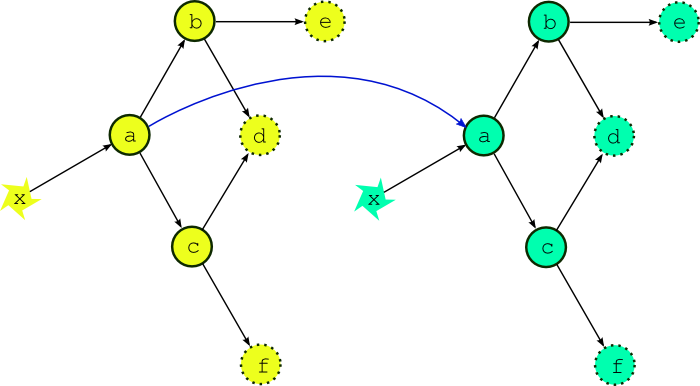
\includegraphics[width=0.4\columnwidth]{resources/tex/dep-two-cycles-linked}
\end{center}

Here's a job schedule for a single cycle of the workflow,
\begin{center}
    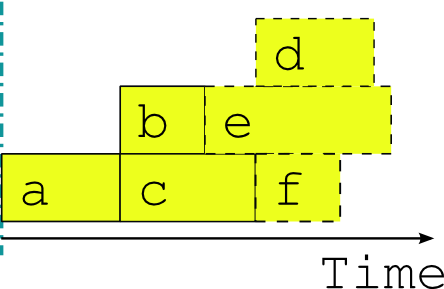
\includegraphics[width=0.17\columnwidth]{resources/tex/timeline-zero.png}
\end{center}

Bar width is proportional to job run time, and the vertical axis has no
meaning.  So {\em b} and {\em c} start running at the same time,
immediately after {\em a} finishes, and so on.  The job schedule for repeatedly
cycling the same workflow is shown below, for cylc (top) and a traditional
fixed-cycle scheduler (bottom) 

\begin{center}
    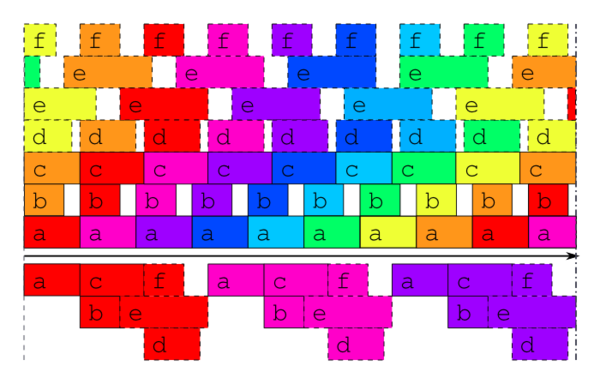
\includegraphics[width=0.5\columnwidth]{resources/tex/timeline-two}
\end{center}

The different colours represent different cycle points.  Cylc automatically
interleave cycles for faster scheduling throughput. In this case cylc is
running tasks from four different cycle points at once, most of the time. The
optimal result is shown (the white time-gaps between tasks are are required by
the dependency relationshionships). This assumes sufficient compute resource to
run every task as soon as its inputs are satisified. But if a task is delayed
(in a batch scheduler queue or otherwise) the system organically adapts, and
the rest of the workflow will carry on as dependencies allow.
